\mysubsection{Interface Homme $ \leftrightarrow $ Machine}\label{res_IHM}

L’interface est composé par une fenêtre où les utilisateurs réalisent les différents mouvements qui composent le jeu. De plus, elle doit recevoir les paramètres concernant la construction du tableau et l’identification des joueurs. Ainsi, l’interface est composé par trois fenêtres principales que sont ouvertes séquentiellement. 

\subsubsection{Première fenêtre: Paramètres du tableau}\label{Fen1}

\begin{figure}[H]
	\begin{center}
		\captionsetup{justification=centering,margin=1cm}	
		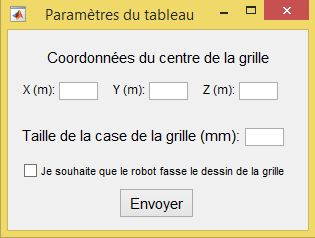
\includegraphics[width=7cm]{./parametres_tableau.jpg}
		\caption{Fenêtre que reçoit les paramètres du tableau}
		\label{fig:Fen1}
	\end{center}
\end{figure}

La position de l’outil et de chaque élément du jeu est décrit dans le repère de la base du robot. Cette fenêtre reçoit les positions du centre du tableau dans le repère de la base du robot. Par ailleurs, pour définir complètement le tableau, la taille de la case de la grille doit être déterminé. Par convention, on a adopté la position initiale du robot comme le centre X et Y du tableau et avec la hauteur Z égal à la taille de la case de la grille. De plus, cette fenêtre offre une option pour calculer le couple et la trajectoire de l’outil génère pour dessiner la grille du tableau. 
 

\subsubsection{Deuxième fenêtre: Utilisateurs}\label{Fen2} 

\begin{figure}[H]
	\begin{center}	
		\captionsetup{justification=centering,margin=1cm}
		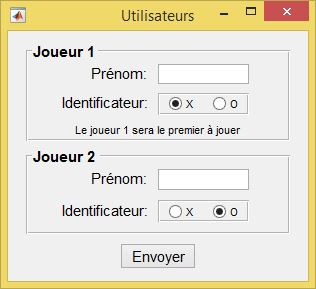
\includegraphics[width=7cm]{./utilisateurs.jpg}
		\caption{Fenêtre que reçoit l'identification des utilisateurs}
		\label{fig:Fen2}
	\end{center}
\end{figure}
\newpage
Pour dérouler le jeu entre deux différents utilisateurs, on a créé une fenêtre que reçoit les paramètres d’identification de chaque joueur, comme son prénom et le symbole associé à chaque joueur. Par convention, on a adopté que le jeu est initié par le joueur 1. 

\subsubsection{Troisième fenêtre: Jeu de Morpion}\label{Fen3}

\begin{figure}[H]
	\begin{center}	
		\captionsetup{justification=centering,margin=1cm}
		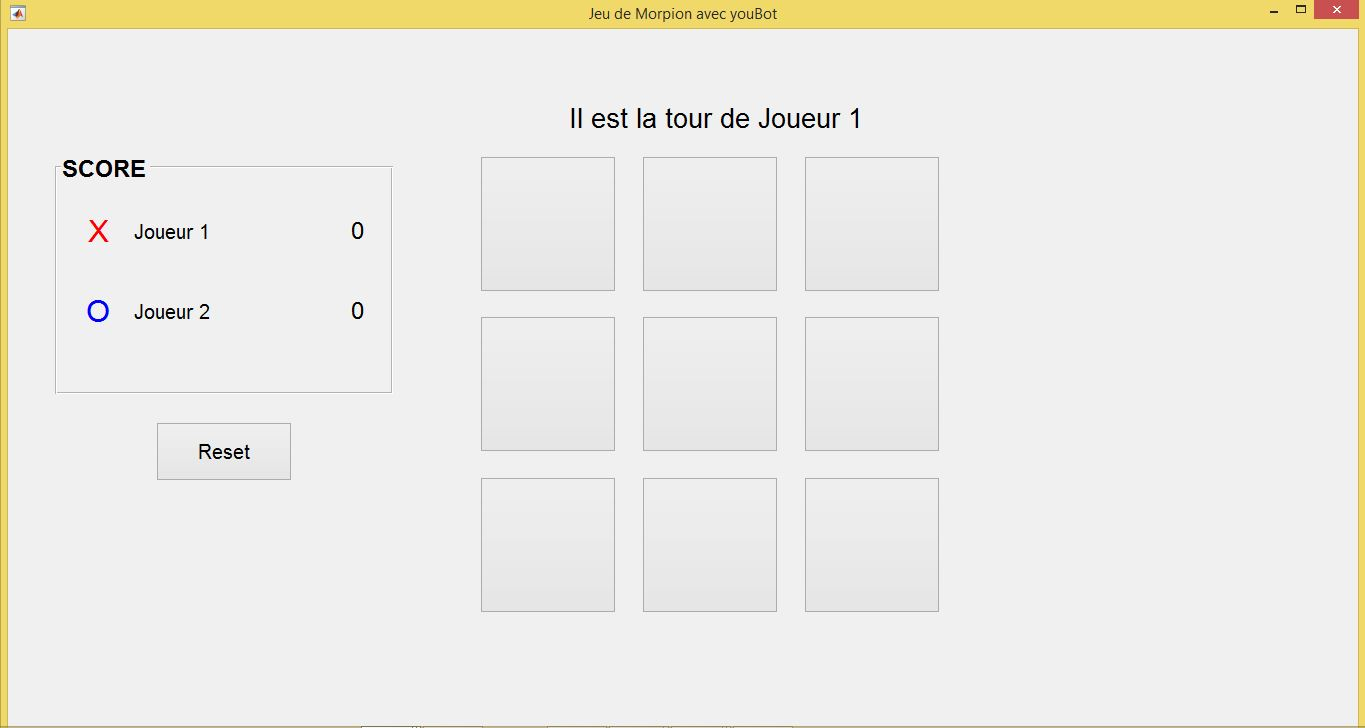
\includegraphics[width=0.9\textwidth]{./jeu_de_morpion.jpg}
		\caption{Fenêtre que reçoit les mouvements du jeu de Morpion}
		\label{fig:Fen3}
	\end{center}
\end{figure}

Cette fenêtre reçoit les mouvements souhaités par chaque joueur. Lorsque le joueur clique sur une case souhaitée, les fonctions de calcul de trajectoire et couple sont appelés et la trajectoire à être exécuté par le robot avec les déplacements sur les  cases du tableau et le dessin du symbole de chaque joueur est tracé sur un graphique 3D.

\begin{figure}[H]
	\begin{center}	
		\captionsetup{justification=centering,margin=1cm}
		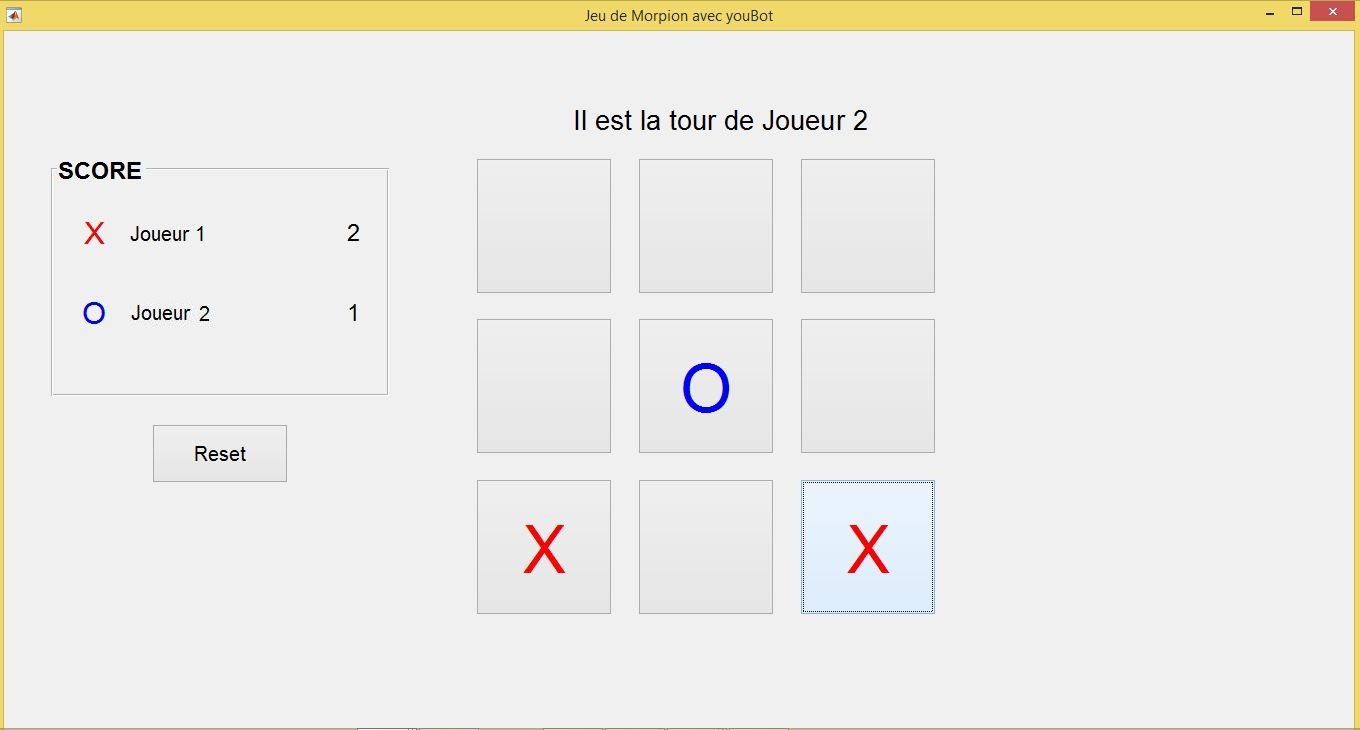
\includegraphics[width=0.9\textwidth]{./Jeu2a1.jpg}
		\caption{Tableau du jeu avec les mouvements des joueurs}
		\label{fig:Jeu}
	\end{center}
\end{figure}

\begin{figure}[H]
	\begin{center}
		\captionsetup{justification=centering,margin=1cm}	
		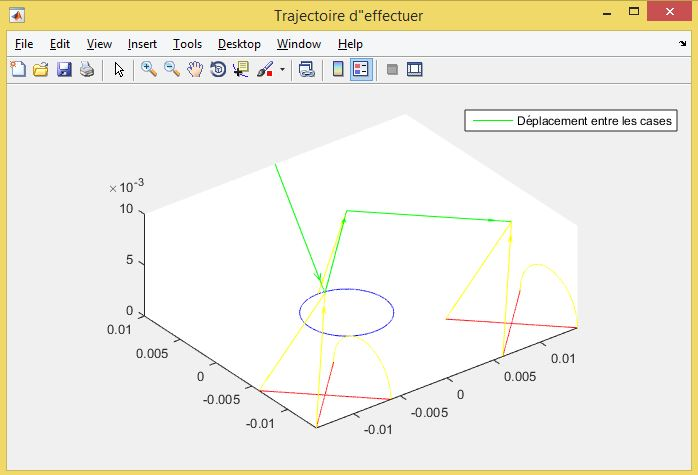
\includegraphics[width=0.9\textwidth]{./grafico.jpg}
		\caption{Graphique 3D que décrit la trajectoire du robot pour faire les mouvements du jeu}
		\label{fig:graphique}
	\end{center}
\end{figure}

Ainsi, ce graphique permet la visualisation du mouvement que le robot fera dans une mise en oeuvre réel du jeu. Comme l’activité d'intégration et synchronisation du module de commande avec l’interface n’est pas été fini, les courbes tracées dans le graphique sont concernant seulement le résultat de la génération de trajectoire, au lieu de la position finale généré par le module de commande calculée à partir de la trajectoire souhaitée. Cependant, comme le module de commande est déjà bien réglé et mis en oeuvre, pour un travail futur suffira de bien régler la synchronisation. 

Quand un tour du jeu est terminé, l’interface annonce le gagnant ou un possible match nul et elle offre aux utilisateurs l’option d’initier un nouveau tour. Si un nouveau tour est initié, le score de chaque joueur est calculé et actualisé sur le panneau de résultats à gauche de l’interface. De plus, il existe l’option de redémarrer un tour en cliquant sur le bouton Reset.



\begin{figure}[H]
	\centering
	
	\begin{minipage}[b]{0.45\textwidth}
		
		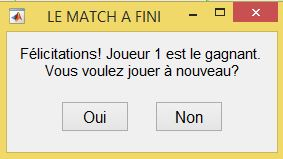
\includegraphics[width=\textwidth]{./match_termina.jpg}
	\end{minipage}
	\hfill
	\begin{minipage}[b]{0.45\textwidth}
		
		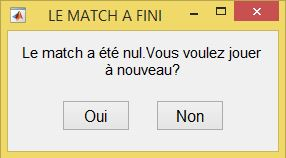
\includegraphics[width=\textwidth]{./match_nul.jpg}
	\end{minipage}
	\captionsetup{justification=centering,margin=1cm}
	\caption{Option d’initier un nouveau tour quand un match finit}
	\label{fig:match}
\end{figure}
\pagebreak



%	\begin{multicols}{2}
%
%	\begin{figure}	
%		
%	\end{figure}
%	\begin{figure}
%		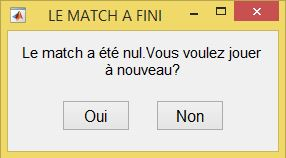
\includegraphics[width=0.\textwidth]{./match_nul.jpg}
%	\begin{figure}
%		\caption{Option d’initier un nouveau tour quand un match finit}
%		\label{fig:match}
%
%\end{multicols}